\chapter{Уақытша күрделілігі}

\index{уақытша күрделілігі}

Алгоритмдердің тез жұмыс істеуінің спорттық бағдарламалауда маңызы зор.
Әдетте есепті баяу шығаратын алгоритмді ойлап табу жеңіл-ақ.
Ал сол есепті тез шығаратын алгоритмді ойлап табу қиынға соғады.
Егер алгоритм өте баяу болса, ол есептен аз немесе нөл ұпай алады.

Алгоритмнің \key{уақытша күрделілігі} -- берілген енгізу бойынша
алгоритмнің қанша уақытта жұмыс жасайтындығының мөлшері. 
Уақытша күрделілігін енгізу бойынша функциямен көрсетеді 
және оны жазғанда $O(\cdots)$ нотациясымен белгілейді. Алдағы уақытта бұған қайта ораламыз.
Уақытша күрделілігін есептеу арқылы біз алгоритмді жазбастан бұрын оның есеп шығару үшін
жылдамдығы жеткілікті дәрежеде екеніне көз жеткізе аламыз.

\section{Есептеу ережелері}

Алгоритмнің уақытша күрделілігі $O(\cdots)$ түрінде белгіленеді, мұндағы көп нүкте қандай да бір функцияны білдіреді.
Әдетте, $n$ айнымалысы енгізудің өлшемін көрсетеді.
Мысалы, егер енгізу сандар жиыны болса, 
$n$ оның өлшемін көрсетеді. Егер жол болса, 
$n$ оның ұзындығын көрсетеді.

\subsubsection{Қайталымдар}

Алгоритмнің баяу болуының әдеттегі себебі -- 
енгізу бойынша өтетін кірістірілген циклдардың көп болуы.
Егер $k$ кірістірілген цикл болса,
уақытша күрделілігі $O(n^k)$-ға тең. 

Мысалы, төмендегі кодтың уақытша күрделілігі -- $O(n)$:
\begin{lstlisting}
for (int i = 1; i <= n; i++) {
    // code
}
\end{lstlisting}

Ал келесі кодтың уақытша күрделілігі -- $O(n^2)$:
\begin{lstlisting}
for (int i = 1; i <= n; i++) {
    for (int j = 1; j <= n; j++) {
        // code
    }
}
\end{lstlisting}

\subsubsection*{Шаманың реті}

Уақытша күрделілігі бізге циклдың ішінде алгоритмнің
қанша рет жұмыс жасайтынын көрсетпейді. Негізінен ол бізге
шаманың ретін ғана көрсетеді.
Төмендегі мысалдарда алгоритмнің циклы $3n$, $n+5$
және $\lceil n/2 \rceil$ итерация жасайтын болса да, 
олардың уақытша күрделілігі $O(n)$ болады.


\begin{lstlisting}
for (int i = 1; i <= 3*n; i++) {
    // code
}
\end{lstlisting}

\begin{lstlisting}
for (int i = 1; i <= n+5; i++) {
    // code
}
\end{lstlisting}

\begin{lstlisting}
for (int i = 1; i <= n; i += 2) {
    // code
}
\end{lstlisting}


Ал мына мысалда уақытша күрделілігі $O(n^2)$-не тең, себебі $1 + 2 + 3 + \cdots + n = \frac{n*(n+1)}{2}$ және $O(\frac{n^2}{2}+\frac{n+1}{2}) = O(n^2)$ (алдағы уақытта кеңірек тоқталамыз):

\begin{lstlisting}
for (int i = 1; i <= n; i++) {
    for (int j = i+1; j <= n; j++) {
        // code
    }
}
\end{lstlisting}



\subsubsection*{Бөлімдер}

Егер кодтағы уақытша күрделілігі бірнеше бөлімдерден тұратын болса,
онда жалпы уақытша күрделілігі оның ең баяу бөліміне тең болады. 
Себебі кодтағы ең баяу бөлім әдетте 
кодтың тар өткеліне айналады. Егер сол баяу бөлімді 
тұрақты санға көбейтетін болсақ, оны өшіре салуға болады 
(яғни $O(3n)=O(n)$).


Мысалы, төмендегі код үш бөлімнен тұрады: 
$O(n)$, $O(n^2)$ және $O(n)$.
Демек жалпы уақытша күрделілігі $O(n^2)$-ге тең.

\begin{lstlisting}
for (int i = 1; i <= n; i++) {
    // code
}
for (int i = 1; i <= n; i++) {
    for (int j = 1; j <= n; j++) {
        // code
    }
}
for (int i = 1; i <= n; i++) {
    // code
}
\end{lstlisting}

\subsubsection*{Бірнеше айнымалылар}

Кейде алгоритмнің уақытша күрделілігі бірнеше факторларға тәуелді болады.
Сол себепті де уақытша күрделілігінде бірнеше айнымалылар кездеседі.

Төмендегі кодтың уақытша күрделілігі $O(nm)$-ға тең:

\begin{lstlisting}
for (int i = 1; i <= n; i++) {
    for (int j = 1; j <= m; j++) {
        // code
    }
}
\end{lstlisting}

\subsubsection*{Рекурсия}

Рекурсиялық функцияның уақытша күрделілігі функцияның 
қанша рет шақырылғанына және бір шақырылымның уақытша күрделілігіне 
байланысты болады. 
Ал қорытынды уақытша күрделілігі олардың көбейтіндісіне тең келеді.

Мысалға келесі рекурсиялық функцияны қарастырайық:
\begin{lstlisting}
void f(int n) {
    if (n == 1) return;
    f(n-1);
}
\end{lstlisting}
$\texttt{f}(n)$ функциясын шақыру $n$ рет сол функцияны орындайды
және әрбір шақырудың уақытша күрделілігі $O(1)$ болады. 
Демек қорытынды уақытша күрделілігі $O(n)$-ға тең.

Келесі мысалға назар аударайық:
\begin{lstlisting}
void g(int n) {
    if (n == 1) return;
    g(n-1);
    g(n-1);
}
\end{lstlisting}
Бұл жерде әр функция шақырылуы $n \neq 1$ болған кезде функцияны 2 рет шақырады.
Егер біз $g(n)$ функциясын шақырсақ, ол 2 $g(n-1)$ функциясын шақырады.
Ал $g(n-1)$ болса, 4 $g(n-2)$ функциясын шақыратын болады. 
Дәл солай кете берсек, бізде төмендегідей кесте шығады:

\begin{center}
\begin{tabular}{rr}
Функция & неше рет шақырылды \\
\hline
$g(n)$ & 1 \\
$g(n-1)$ & 2 \\
$g(n-2)$ & 4 \\
$\cdots$ & $\cdots$ \\
$g(1)$ & $2^{n-1}$ \\
\end{tabular}
\end{center}
Осыған байланысты біздің уақытша күрделілігіміз:
\[1+2+4+\cdots+2^{n-1} = 2^n-1 = O(2^n).\]

\section{Күрделілік кластары}

\index{күрделілік кластары}

Төмендегі тізімде алгоритмдердің уақытша күрделіліктеріне сипаттама беріледі:

\begin{description}
\item[$O(1)$] --
\index{тұрақты алгоритм} 
\key{Алгоритмнің} уақытпен жұмыс істеу кезеңі кіріс деректердің көлеміне байланысты болмайды. Бұның қарапайым мысалы ретінде сол бойынша жауапты есептеп шығаратын айқын формуланы  алуға болады. 

\item[$O(\log n)$] --
\index{логаримфдік алгоритм} 
\key{Логарифмдік алгоритмде} 
кіріс деректердің көлемі әр қадам сайын әдетте екіге кеміп отырады. Жұмыс істеу уақыты кіріс деректердің көлеміне байланысты болады. Өйткені  мұндай алгоритмге логаримфдік жұмыс уақыты тән.
Себебі $n$-ді екіге бөле берсек, ақырында $\log n$ рет бөлуден кейін 1-ге жетеміз.

\item[$O(\sqrt n)$] --
\index{квадратты түбір алгоритмдер}
\key{Уақытша күрделілігі} $O(\sqrt n)$ алгоритмдер $O(\log n)$–нан баяуырақ, бірақ $O(n)$-нен жылдамырақ болады.
Квадратты түбірдің ерекше қасиеті -- 
$\sqrt n = n/\sqrt n$ болуында. Демек $n$ элементті 
$O(\sqrt n)$ элементтер бойынша $O(\sqrt n)$ бөлікке бөлшектей аламыз.

\item[$O(n)$] --
\index{сызықтық уақыт алгоритм}
\key{Сызықтық} алгоритм кіріс деректерді тұрақты уақытта өтіп шығады.
Бұл көбіне алгоритмнің ең жақсы ықтимал уақытша күрделілігі болып келеді.
Себебі жауапты алу үшін әр элементке тым болмаса бір рет жүгіну керек болады. 

\item[$O(n \log n)$] --
\key{Алгоритмнің} мұндай уақытша күрделілігі әдетте оның кіріс деректерді сұрыптайтын білдіреді. Себебі сұрыптау алгоритмдерінің 
ең тиімді уақытша күрделілігі $O(n \log n)$-ге тең. Алгоритмде әр операция $O(\log n)$ уақыт алатын деректер құрылымы қолданылатын басқа мүмкіндіктер де бар. 

\item[$O(n^2)$] --
\index{квардаттық алгоритм}
\key{Квадраттық} алгоритм әдетте екі
кірістірілген циклден тұрады. Кіріс элементтерінің барлық жұптарын
өтіп шығу $O(n^2)$ уақытты алады.

\item[$O(n^3)$] --
\index{кубтық алгоритм}
\key{Кубтық} алгоритм әдетте үш
кірістірілген циклден тұрады.
Кіріс элементтердің барлық үштіктерін
өтіп шығу $O(n^3)$ уақытты алады.

\item[$O(2^n)$] --
\key{Алгоритмнің} мұндай
уақытша күрделілігі әдетте алгоритмнің кіріс деректер жиынының барлық 
ішжиынын өтіп шыққанына нұсқайды. Мысалы, $\{1,2,3\}$ элементтерінің барлық ішжиыны
$\emptyset$, $\{1\}$, $\{2\}$, $\{3\}$, $\{1,2\}$,
$\{1,3\}$, $\{2,3\}$ және $\{1,2,3\}$ болады.

\item[$O(n!)$] --
\key{Алгоритмнің} 
мұндай уақытша күрделілігі әдетте алгоритмнің кіріс элементтердің барлық 
алмастыруларын өтіп шыққанына нұсқайды. Мысалы, $\{1,2,3\}$ элементтердің барлық алмастыруы
$(1,2,3)$, $(1,3,2)$, $(2,1,3)$, $(2,3,1)$,
$(3,1,2)$ және $(3,2,1)$ болады.

\end{description}

\index{полиномдық алгоритм}
Уақытша күрделілігі ең көп дегенде $O(n^k)$-не тең болатын алгоритм полиномдық алгоритм деп аталады. Мұндағы $k$ тұрақты.
$O(2^n)$ және $O(n!)$ алгоритмдерінен басқа барлық
алгоритм полиномдық алгоритм болып есептеледі. 
Іс жүзінде мұндай алгоритмдер \emph{тиімді}, себебі k көп жағдайда аз болады.

\index{NP-қиын есептер}

Бұл кітаптағы алгоритмдердің көбі - полиномдық алгоритмдер.
Дегенмен кейбір маңызды есептерді полиномдық уақытта шығару мүмкін емес. Басқаша айтқанда, ондай есептерді ешкім тиімді шығара алмайды. Бұл есептердің жиынын \key{NP-қиын} есептер деп атайды және оларды шешетін полиномдық алгоритмдерді әзірше ешкім білмейді \footnote{
Осы тақырып бойынша классикалық кітаптардың бірі --
М.Р.Гэрей мен Д.С.Джонсонның
\emph{Computers and Intractability: A Guide to the Theory
of NP-Completeness} атты кітабы \cite{gar79}.}.

\section{Тиімділікті бағалау}

Алгоритмнің уақытша күрделілігін есептей отырып, 
алгоритмді жазбас бұрын оның есеп үшін жеткілікті дәрежеде тиімді екенін тексеріп алуға болады.
Бағалауды бастамас бұрын қазіргі заманғы 
компьютер бір секундта жүз миллиондаған операция
орындай алатынын ескеру қажет.

Мысалы, бір есептің уақыт шегі 1 секунд, 
ал енгізудің өлшемі $n=10^5$ дейік.
Егер уақытша күрделілігі $O(n^2)$ болса, алгоритм $(10^5)^2=10^{10}$ операция жасайды.
Бұл алгоритм ең кемінде 10 секунд алады.  
Есепті шешу үшін тым баяу болғандықтан, 
қолданысқа қолайлы емес екенін байқаймыз.

Екінші жағынан, берілген енгізудің өлшемі арқылы
есепті шығаратын алгоритмнің уақытша күрделілігін \emph{болжай}
аламыз.
Келесі кестеде уақыт шегі 1 секунд болатын есептерге
көмектесетін алгоритмдердің болжамды бағалары берілген.

\begin{center}
\begin{tabular}{ll}
енгізу өлшемі & талап етілетін уақытша күрделілігі \\
\hline
$n \le 10$ & $O(n!)$ \\
$n \le 20$ & $O(2^n)$ \\
$n \le 500$ & $O(n^3)$ \\
$n \le 5000$ & $O(n^2)$ \\
$n \le 10^6$ & $O(n \log n)$ немесе $O(n)$ \\
$n$ тым үлкен & $O(1)$ немесе $O(\log n)$ \\
\end{tabular}
\end{center}

Мысалы, егер енгізу өлшемі $n=10^5$ болса,
онда алгоритмнің уақытша
күрделілігі $O(n)$ немесе $O(n \log n)$ болады деп күтілуде.
Бұл мағлұмат алгоритмдерді жобалауға көмек береді, өйткені
уақытша күрделілігі баяу алгоритмдерді қарастырған тиімсіз.

\index{тұрақты фактор}

Уақытша күрделілігі кодтың тиімділігін
бағалайтынын естен шығармау керек. Ол кодтың нақты
неше операция жасайтынын көрсетпейді және ол 
\emph{тұрақты факторларды} жасырады. Мысалы,
$O(n)$ жасайтын алгоритм шын мәнінде 
$n/2$ немесе $5n$ операция жасауы мүмкін. 
Бұл алгоритмнің жұмыс жасау уақытына 
сөзсіз әсер етеді.

\section{Ішжиымдардың ең жоғары қосындысы}

\index{ішжиымдардың ең жоғары қосындысы}

Бір есептің шығарылу барысында уақытша күрделілігі 
әртүрлі бірнеше алгоритмдер кездеседі. Бұл бөлімде
классикалық есепті $O(n^3)$ уақытта шығару жолын
талқылаймыз. Дегенмен жақсырақ алгоритмді 
жобалау арқылы бұл есепті $O(n^2)$
немесе одан анағұрлым тиімдірек $O(n)$ уақытта шешуге болады.

Бізге өлшемі $n$ болатын жиым берілген.
Оның \key{ішжиымдарының ең жоғары қосындысын}
табуымыз керек. Басқаша айтқанда 
жиымдағы көршілес болатын тізбектердің
ең жоғары қосындысының мәнін табу\footnote{Дж. Бэнтлейдің \emph{Programming Pearls} \cite{ben86} кітабы есепті танымал етті.} қажет.
Егер жиымда теріс сандар болса, бұл есеп
қызығырақ шығарылады. Мысалы, мына жиымда
\begin{center}
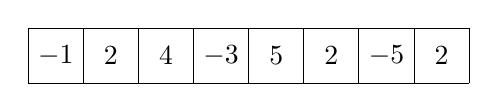
\begin{tikzpicture}[scale=0.7]
\draw (0,0) grid (8,1);

\node at (0.5,0.5) {$-1$};
\node at (1.5,0.5) {$2$};
\node at (2.5,0.5) {$4$};
\node at (3.5,0.5) {$-3$};
\node at (4.5,0.5) {$5$};
\node at (5.5,0.5) {$2$};
\node at (6.5,0.5) {$-5$};
\node at (7.5,0.5) {$2$};
\end{tikzpicture}
\end{center}
\begin{samepage}
ішжиымдардың максималды қосындысы $10$ болады:
\begin{center}
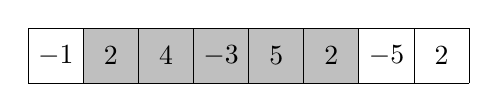
\begin{tikzpicture}[scale=0.7]
\fill[color=lightgray] (1,0) rectangle (6,1);
\draw (0,0) grid (8,1);

\node at (0.5,0.5) {$-1$};
\node at (1.5,0.5) {$2$};
\node at (2.5,0.5) {$4$};
\node at (3.5,0.5) {$-3$};
\node at (4.5,0.5) {$5$};
\node at (5.5,0.5) {$2$};
\node at (6.5,0.5) {$-5$};
\node at (7.5,0.5) {$2$};
\end{tikzpicture}
\end{center}
\end{samepage}

Бос ішжиымның қосындысы $0$ деп санайық.
Есеп шарты бойынша бос ішжиым алуға болатынын ескеруіміз керек. Демек ішжиымдардың ең жоғары қосындысы кем 
дегенде $0$ болады.

\subsubsection{1-алгоритм}

Барлық ішжиымдарды қарап, олардың қосындысын
бір айнымалыға сақтау арқылы бұл есепті ең оңай алгоритммен шығаруға болады.
Осы алгоритмді төмендегі код іске асырады:

\begin{lstlisting}
int best = 0;
for (int a = 0; a < n; a++) {
    for (int b = a; b < n; b++) {
        int sum = 0;
        for (int k = a; k <= b; k++) {
            sum += array[k];
        }
        best = max(best,sum);
    }
}
cout << best << "\n";
\end{lstlisting}

\texttt{a} мен \texttt{b} итераторлары ішжиымның 
бірінші және соңғы индекстері ретінде қарастырылады.
Араларындағы элементтердің ең аз қосындысын \texttt{sum} айнымалысында, 
ал ең көп қосындыны \texttt{best} айнымалысында
 сақтаймыз. 

Бұл алгоритмнің уақытша күрделілігі $O(n^3)$, себебі 
алгоритмде үш кірістірілген цикл енгізуді өтіп шығады.

\subsubsection{2-алгоритм}

1-алгоритмнен бір циклді алып тастау арқылы оны тиімдірек 
жобалай аламыз. Ішжиымның соңғы индексі өзгерген сәтте
ғана қосындыны санауға болады.  
Нәтижесінде код төмендегідей болып өзгереді:

\begin{lstlisting}
int best = 0;
for (int a = 0; a < n; a++) {
    int sum = 0;
    for (int b = a; b < n; b++) {
        sum += array[b];
        best = max(best,sum);
    }
}
cout << best << "\n";
\end{lstlisting}
Бұл өзгерістен кейін уақытша күрделілігі $O(n^2)$ болады.

\subsubsection{3-алгоритм}

Бір қарағанда мүмкін еместей болып көрінгенімен бұл есепті $O(n)$ уақытта шығаруға болады
\footnote{\cite{ben86}-еңбекте бұл сызықтық уақыт алгоритмнің  Дж.Б.Каданеге қатыстылығы көрсетіледі.
Оны кейде \key{Кадане алгоритмі} деп те атайды.}.
Нақтырақ айтқанда, бір ғана цикл арқылы шығара аламыз. Идеясы әрбір индекс үшін
сол жерден бітетін ең жоғары ішжиымның қосындысын есептеуге, ал кейін солардың
максимумын табуға негізделеді.

$k$ индексінде бітетін ең жоғары ішжиым есебін қарастырайық.
Бұл жерде екі нұсқа бар:
\begin{enumerate}
\item Ең жоғары ішжиым индексі тек $k$ болатын элементтен тұрады.
\item Ең жоғары ішжиым $k-1$ индексінде аяқталатын ішкі жиымнан және одан кейінгі $k$ индексіндегі элементтен тұрады.
\end{enumerate}

Екінші жағдайда қосындысы ең жоғары ішжиымды 
іздейтіндіктен, $k-1$ позициясында аяқталатын ішжиымның 
қосындысы да ең жоғары болуы керек.
Демек бұл есептің тиімді шығарылу жолы
солдан оңға қарай әр индекске сол жерден бітетін
ең жоғары қосындыны есептеу болмақ.

Бұл жағдайда төмендегі алгоритм коды тиімді:
\begin{lstlisting}
int best = 0, sum = 0;
for (int k = 0; k < n; k++) {
    sum = max(array[k],sum+array[k]);
    best = max(best,sum);
}
cout << best << "\n";
\end{lstlisting}

Алгоритмді енгізу бойынша бір ғана цикл өтетіндіктен оның уақытша күрделілігі 
$O(n)$ болады және бұл ең тиімді алгоритм саналады.

\subsubsection{Тиімділікті салыстыру}

Енді аталған алгоритмдердің тиімділігін іс жүзінде байқап көрейік.
Төмендегі кестеде үш алгоритмнің $n$ әртүрлі мәндерге тең болғандағы заманауи компьютердегі жұмыс уақыты берілген.

Әр тест кездейсоқ мәндер арқылы құрастырылып, енгізуді оқу уақыты қарастырылмаған.

\begin{center}
\begin{tabular}{rrrr}
Енгізу өлшемі $n$ & 1-алгоритм & 2-алгоритм & 3-алгоритм \\
\hline
$10^2$ & $0.0$ с & $0.0$ с & $0.0$ с \\
$10^3$ & $0.1$ с & $0.0$ с & $0.0$ с \\
$10^4$ & > $10.0$ с & $0.1$ с & $0.0$ с \\
$10^5$ & > $10.0$ с & $5.3$ с & $0.0$ с \\
$10^6$ & > $10.0$ с & > $10.0$ с & $0.0$ с \\
$10^7$ & > $10.0$ с & > $10.0$ с & $0.0$ с \\
\end{tabular}
\end{center}

Бұл кесте егер енгізу өлшемі кішкентай болса,
барлық алгоритм тиімді жұмыс істейтінін көрсетеді.
Алайда енгізу өлшемі ұлғайған сайын, алгоритмдердің жұмыс уақытында үлкен айырмашылық пайда болатынын байқаймыз.
$n=10^4$ болған сәтте 1-алгоритм баяу болса,
$n=10^5$ болғанда 2-алгоритм баяулайды.
Тек 3-алгоритм ғана үлкен енгізулерді бірден
өңдеуге қабілетті.
